\documentclass{article}
\usepackage[utf8]{inputenc}
\usepackage[slovene]{babel}
\usepackage{graphicx}
\usepackage{subfigure}
\usepackage{amsfonts} 
\usepackage{amsmath}

\newcommand{\program}{Finanča matematika} 
\newcommand{\imeavtorja}{Anja Plesec}
\newcommand{\imementorja}{prof.~dr.~ Sergio Cabello Justo, \\ asist. Gašper Domen Romih}
\newcommand{\naslovdela}{Gradientni spust}
\newcommand{\letnica}{2022}

\begin{document}

\thispagestyle{empty}
\noindent{\large
UNIVERZA V LJUBLJANI\\[1mm]
FAKULTETA ZA MATEMATIKO IN FIZIKO\\[5mm]
\program\ -- 2.~stopnja}
\vfill

\begin{center}{\large
\imeavtorja\\[2mm]
{\bf \naslovdela}\\[10mm]
Kratko poročilo pri predmetu Matematika z računalnikom\\[1cm]
Mentor: \imementorja}
\end{center}
\vfill

\noindent{\large
Ljubljana, \letnica}
\pagebreak

\newpage


\section{Gradientni spust}
Gradientni spust je iterativna metoda za iskanje lokalnega minimuma funkcije. To je algoritem, ki se lahko uporablja na različnih področjih. Cilj pa je imeti algoritem s čim manj iteracij. \\

Samo delovanje algoritma je sledeče. Najprej si izberemo začetno točko (initial value) - $x_0 \in \mathbb{R}^n $ in hitrost konvergence (learning rate). Zapišemo stroškovno funkcijo (Loss Function) in jo odvajamo po vseh parametrih. Na ta način dobimo gradient stroškovne funkcije. Izbrano začetku točko nato vstavimo v ta gradient in s pomočjo tega poračunamo velikost naslednjega koraka:
$$ \text{velikost koraka} = \nabla f(x_t) \cdot \text{learning rate} $$
Vrednost novega parametra pa dobimo s pomočjo spodnje formule:
$$ x_1 = x_0 - \text{velikost koraka} \in \mathbb{R}^n$$
Ko izračunamo vrednost $x_1$ postopek ponovimo.\\

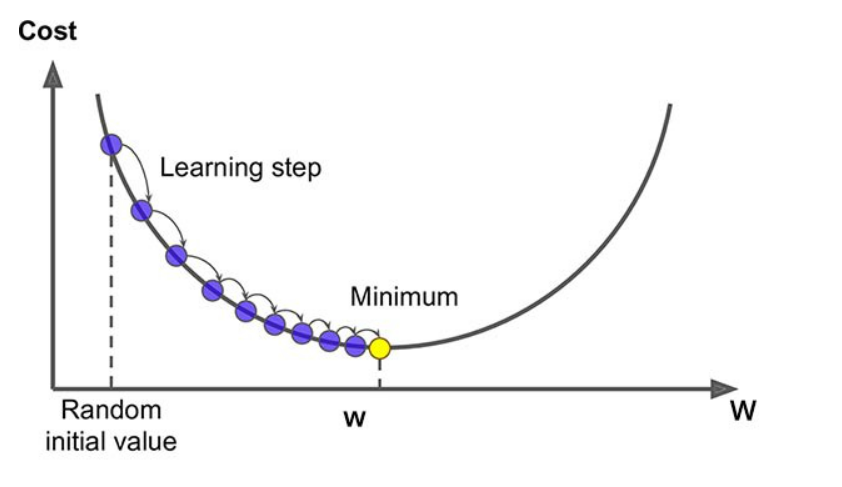
\includegraphics[scale=0.6]{grad_des}
\newline

Splošen algoritem:
\begin{itemize}
\item{Izberemo začetno točko $x_0 \in \mathbb{R}^n $. }
\item{Za $t \geq 0$ predpostavimo, da poznamo $x_0,x_1, \ldots ,x_t $. Naslednji člen določimo s pomočjo enačbe: 
\[ x_{t+1}=x_t - \eta \cdot \nabla f(x_t), \] 
kjer $ \eta$ predstavlja learning rate, $\nabla f(x_t) $ pa gradient funkcije $f$ v točki $x_t$.}
\item{Končamo in vrnemo zadnjo iteracijo.}
\end{itemize}

Težave, ki se pri tem algoritmu pojavijo, so ustrezna izbira vhodnih podatkov. Eden izmed teh je ``learning rate''. Radi bi delali velike korake, kar bi pomenilo manjše število iteracij, vendar se nam lahko zgodi, da s tem zgrešimo našo rešitev in sam algoritem ne vrne prave rešitve. Naslednji izmed vhodnih podatkov je začetna točka $x_0$. Želimo si jo izbrati tako, da je čim bližje optimalni rešitvi, saj bomo zaradi tega potrebovali manj iteracij.\\

Projekt bom izdelala v programu Matlab.

\section{Plan dela}
Za lažji začetek projektne naloge sem pregledala teorijo in na spletu poiskala različne načine uporabe te metode. Da bi čim bolje razumela delovanje tega algoritma sem si v Matlabu pogledala enostaven primer uporabe in sicer za linearno regresijo. Generirala sem 20 naključno izbranih točk potem pa sem s pomočjo algoritma poiskala premico, ki se tem točkam najbolje prilega. Na tem primeru sem spreminjala vhodne podatke in opazovala kako se algoritem odziva.\\

V nadaljevanju bom obravanvala tudi funkcije več spremenljivk in poiskala njihove minumume. Na teh funkcij bom spreminjala vhodne podatke in opazovala kako se algoritem odziva




\end{document}